\section{Schematic}

Raspberry Pi is a single-board computer developed in the United Kingdom by the Raspberry Pi Foundation to promote teaching of basic computer science in schools and in developing countries.The original model clocked at 700Mhz, had composite video output and no wifi, it became popular selling outside its target market for uses such as robotics. 

The first generation (Raspberry Pi 1 Model B) was released in February 2012, followed by the simpler and cheaper Model A. In 2014, the Foundation released a board with an improved design, Raspberry Pi 1 Model B+. These boards are approximately credit-card sized and represent the standard mainline form-factor. Improved A+ and B+ models were released a year later. A "Compute Module" was released in April 2014 for embedded applications. The Raspberry Pi 2, which added more RAM, was released in February 2015.

Raspberry Pi 3 Model B was released in February 2016 with a 1.2 GHz 64-bit quad core processor, on-board 802.11n Wi-Fi, Bluetooth and USB boot capabilities.It has gigabit Ethernet (throughput limited to ca. 300 Mbit/s by the internal USB 2.0 connection) or 2.4 / 5 GHz dual-band 802.11ac Wi-Fi (100 Mbit/s). Other features are Power over Ethernet (PoE) (with the add-on PoE HAT), USB boot and network boot (an SD card is no longer required).
\begin{figure}[ht]
\centering
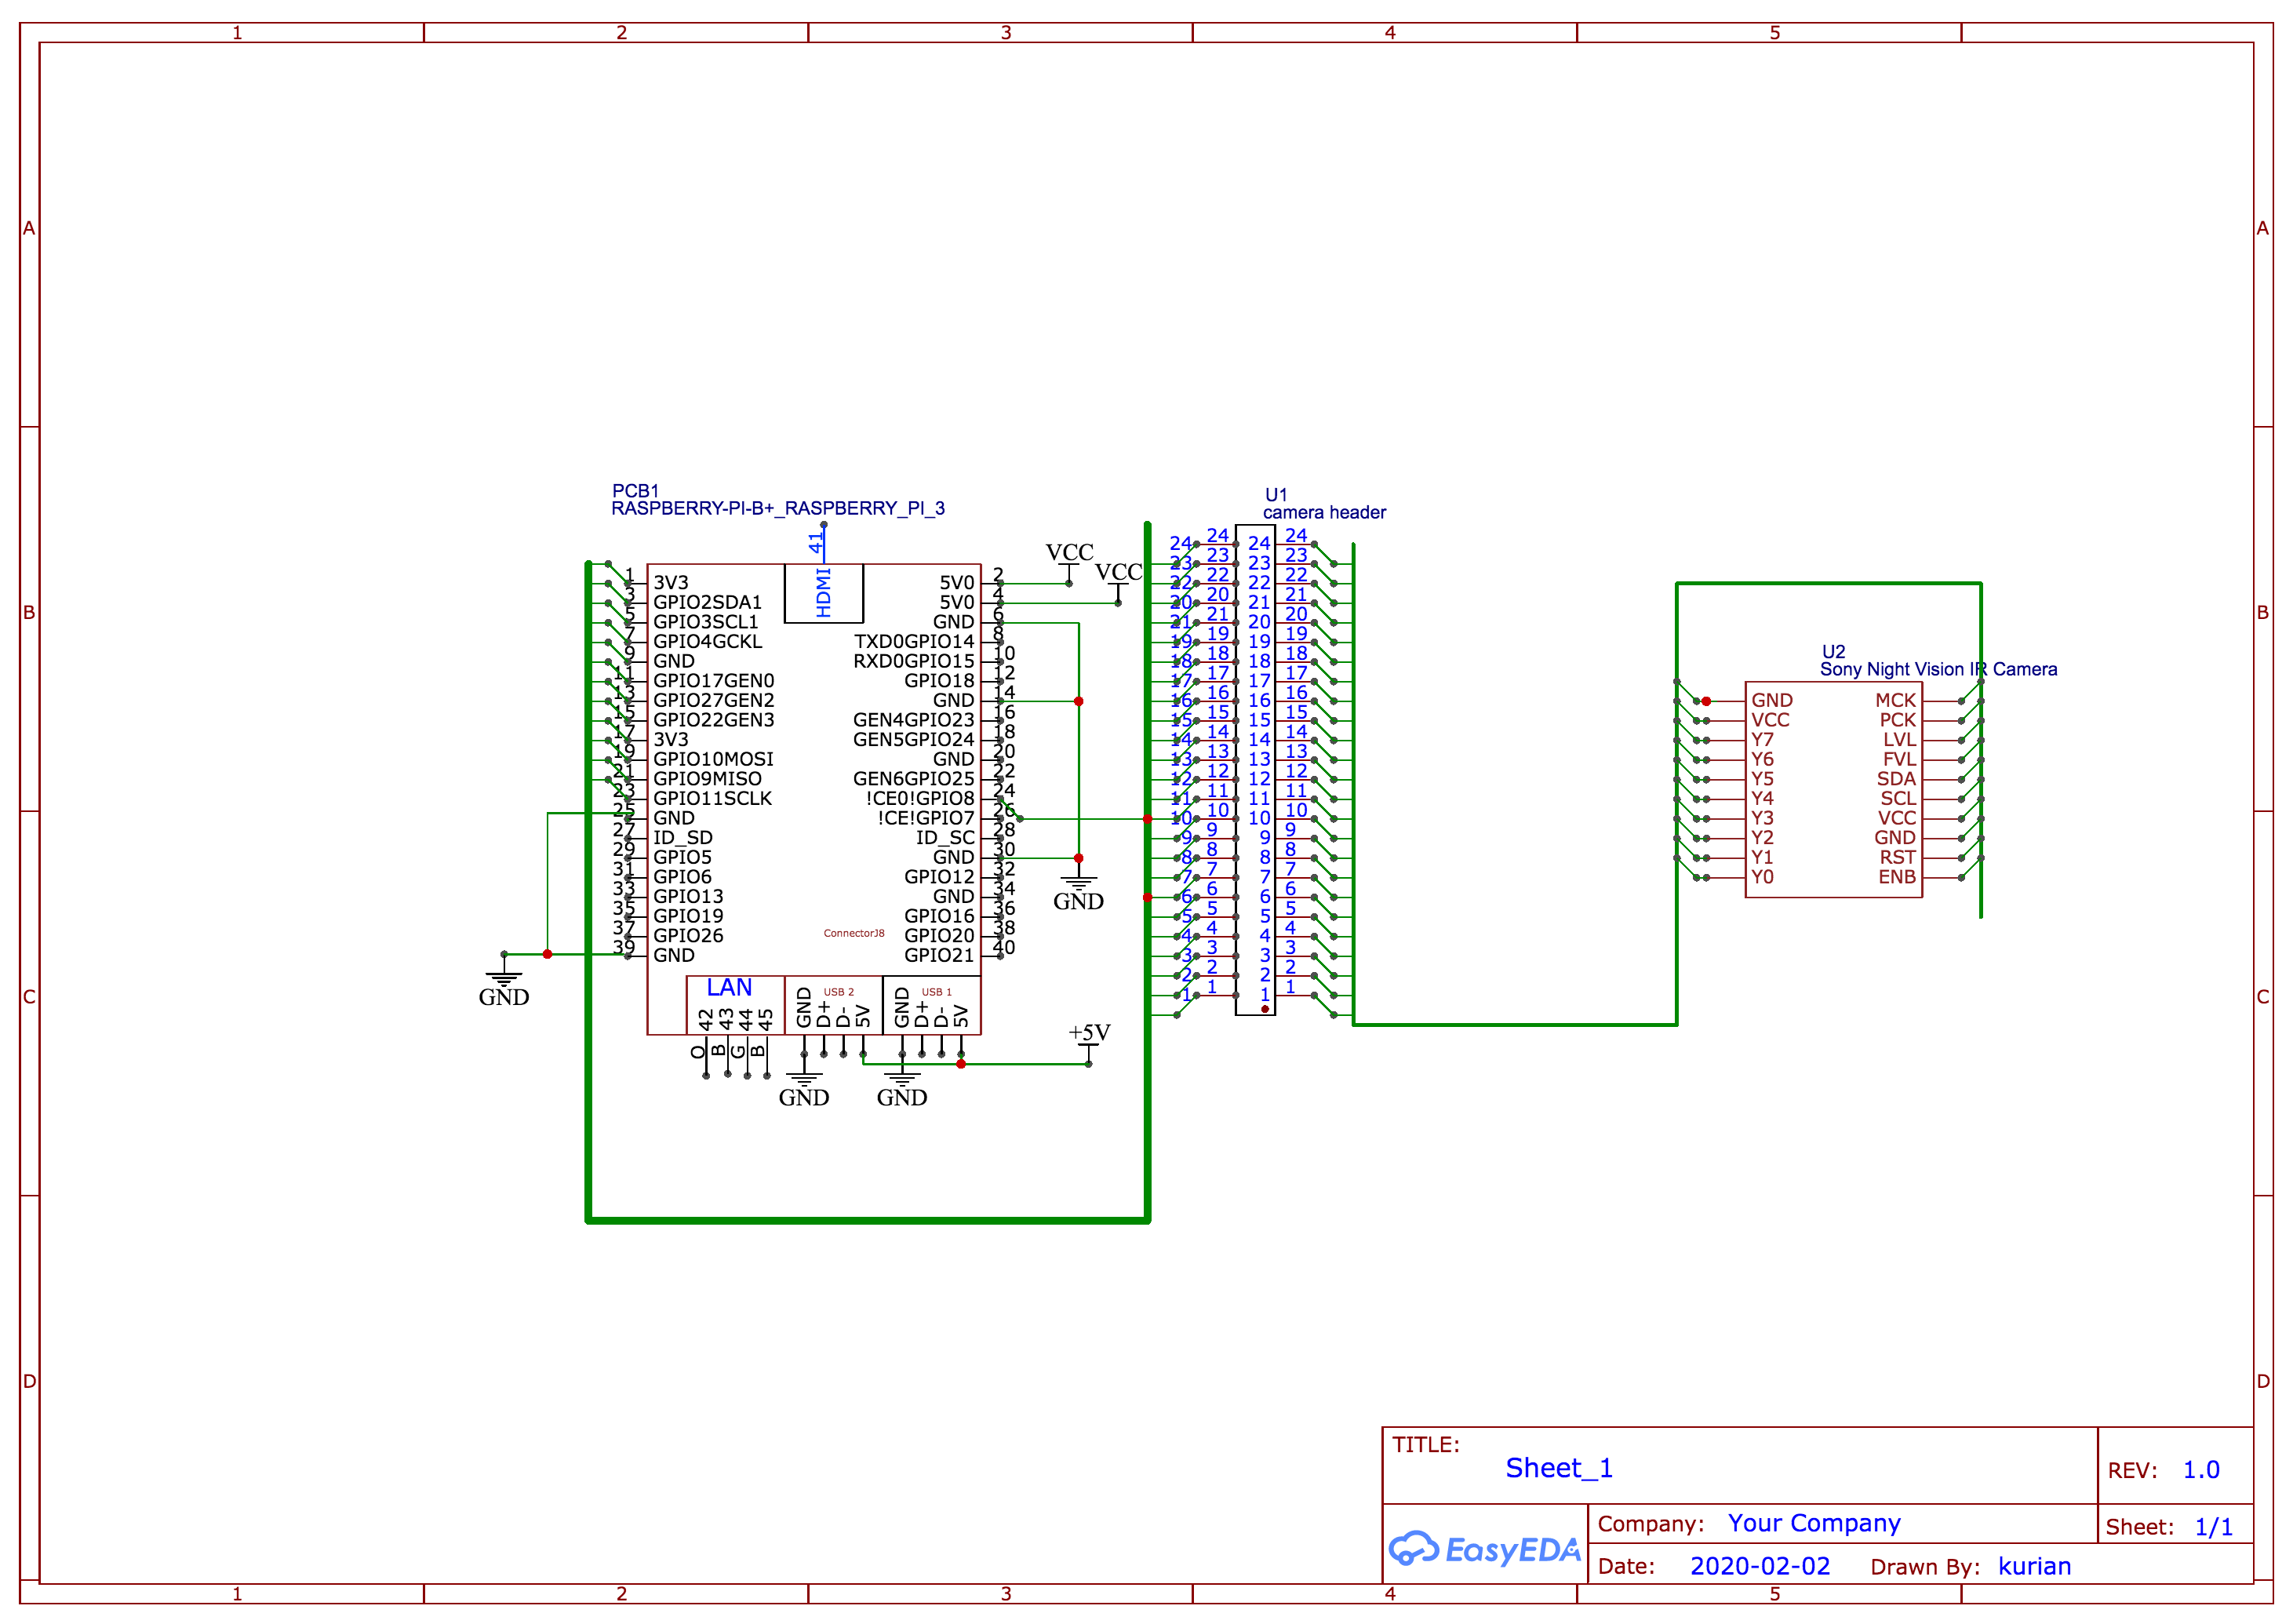
\includegraphics[scale=0.15]{project}
\caption{Schematic of attention tracker}
\end{figure}
